\documentclass[9pt]{beamer}

%~~~~~~~~~~~~~~~~~~~~~~~~~~~~~~~~~~~~~~~~~~~~~~~~~~~~~~~~~~~~~~~~~~~~~~~~~~~~~~
% Use roboto Font (recommended)
\usepackage[sfdefault]{roboto}
\usepackage[utf8]{inputenc}
\usepackage[T1]{fontenc}
%~~~~~~~~~~~~~~~~~~~~~~~~~~~~~~~~~~~~~~~~~~~~~~~~~~~~~~~~~~~~~~~~~~~~~~~~~~~~~~

%~~~~~~~~~~~~~~~~~~~~~~~~~~~~~~~~~~~~~~~~~~~~~~~~~~~~~~~~~~~~~~~~~~~~~~~~~~~~~~
% Define where theme files are located. ('/styles')
\usepackage{styles/fluxmacros}
\usefolder{styles}
% Use Flux theme v0.1 beta
% Available style: asphalt, blue, red, green, gray 
\usetheme[style=green]{flux}
%~~~~~~~~~~~~~~~~~~~~~~~~~~~~~~~~~~~~~~~~~~~~~~~~~~~~~~~~~~~~~~~~~~~~~~~~~~~~~~

%~~~~~~~~~~~~~~~~~~~~~~~~~~~~~~~~~~~~~~~~~~~~~~~~~~~~~~~~~~~~~~~~~~~~~~~~~~~~~~
% Extra packages for the demo:
\usepackage{booktabs}
\usepackage{colortbl}
\usepackage{ragged2e}
\usepackage{schemabloc}
\usepackage{subfigure}
\usepackage{hyperref}
\usepackage[usenames]{color}
%~~~~~~~~~~~~~~~~~~~~~~~~~~~~~~~~~~~~~~~~~~~~~~~~~~~~~~~~~~~~~~~~~~~~~~~~~~~~~~
%~~~~~~~~~~~~~~~~~~~~~~~~~~~~~~~~~~~~~~~~~~~~~~~~~~~~~~~~~~~~~~~~~~~~~~~~~~~~~~
% Informations
\subtitle{\\
\LARGE{CAsimulations: Modelación de dinámicas topológicas } \\
\LARGE{en la propagación de una enfermedad usando}\\
\LARGE{autómatas celulares}}
%\subtitle{The winding number}
\author{Jorge Andres Ibañez Huertas, 
Carlos Isaac Zainea Maya}
\institute{Central University, Bogotá}
\date{\today}
\titlegraphic{Imagenes/logo.png}
%~~~~~~~~~~~~~~~~~~~~~~~~~~~~~~~~~~~~~~~~~~~~~~~~~~~~~~~~~~~~~~~~~~~~~~~~~~~~~~

\begin{document}

% Generate title page
\titlepage

\begin{frame}{Introducción}
Hoy en día existen muchos modelos matemáticos para proyectar el progreso de una enfermedad. Contingencias como la vivida con COVID 19 promueven una mayor comprensión de estos modelos y se crean nuevas teorías en torno a este problema desde diferentes perspectivas.

A pesar de todos los avances realizados hasta el momento, se identifica que no se han tenido en cuenta las interacciones sociales más usuales. Es por esto que podemos preguntarnos por \textbf{¿cuál es el nivel de incidencia de las interacciones sociales en la propagación de una enfermedad?}
\end{frame}

\begin{frame}{Objetivos}
\begin{enumerate}
    \item Proporcionar una herramienta capaz de analizar los fenómenos epidemiológicos a partir de las interacciones sociales en un grupo de individuos.
    \item Proporcionar una metodología para construir modelos epidemiológicos a partir de patrones y reglas lógicas.
    \item Determinar el impacto de las interacciones sociales en la propagación de una enfermedad.
\end{enumerate}
\end{frame}

\begin{frame}
\frametitle{Tabla de Contenidos}
\tableofcontents
\end{frame}

\section{Preliminares}
\subsection{Estudio epidemiológico}
\begin{frame}{Estudio epidemiológico}
La epidemiología es la rama de las ciencias que se encarga de estudiar la ocurrencia y distribución de eventos, estados y procesos relacionados con la salud de distintas poblaciones, con el objetivo de brindar estrategias de control y prevención de problemas de salud relevantes \cite{epiDictionary}.

Uno de los objetos de estudio con mayor importancia en el campo de la epidemiología es la \textbf{cualidad endémica} de la enfermedad, es decir, si la enfermedad afectará a la población por un largo periodo de tiempo o si desaparecerá gradualmente. 
\end{frame}

\begin{frame}{El indicador $\mathcal{R}_0$}
Se define como la cantidad de individuos que infecta el paciente cero en una población completamente susceptible. 

\begin{equation}\label{eq:R0}
 \mathcal{R}_0 = \int_0^\infty b(t)F(t) dt,
\end{equation}

donde $b(t)$ representa la \textbf{cantidad promedio de nuevos contagios} que producirá un individuo infectado durante un tiempo $t$ y $F(t)$, conocida como la función de supervivencia, representa la \textbf{probabilidad de que un individuo recién infectado se mantenga en ese estado} durante al menos un tiempo $t$ \cite{conceptOfR0, perspectivesOnR0}.

En general, si $\mathcal{R}_0<1$ la enfermedad desaparecerá paulatinamente y sí $\mathcal{R}_0>1$, podríamos estar ante un caso de endemia.
\end{frame}

\subsection{Modelos compartimentales: Modelos SIS y SIR}
\begin{frame}{Modelos compartimentales}
Tradicionalmente, se han utilizado modelos de compartimientos para elaborar análisis epidemiológicos. En estos modelos, cada individuo perteneciente a la población de estudio, es clasificado en uno de $n$ posibles ''compartimientos'', según su estado de salud.

Generalmente, se consideran tres estados en las que podemos dividir a la población en el tiempo: Los que pueden contraer la enfermedad, los que se infectan y los que se recuperan. Los modelos que consideran estas variaciones se conocen como los modelos SIS y SIR.

\textbf{Nota:} Usaremos las versiones con tamaño de población constante de los modelos SIS y SIR. Se espera que en futuras investigaciones se profundice en poblaciones de tamaño variable.
\end{frame}

\begin{frame}{Modelos compartimentales: Modelos SIS y SIR}
Diagramas compartimentales para los modelos SIS y SIR en sus versiones con muerte causada por enfermedad:\\

\begin{minipage}{0.46\textwidth}
\begin{figure}[h]
  \centering
    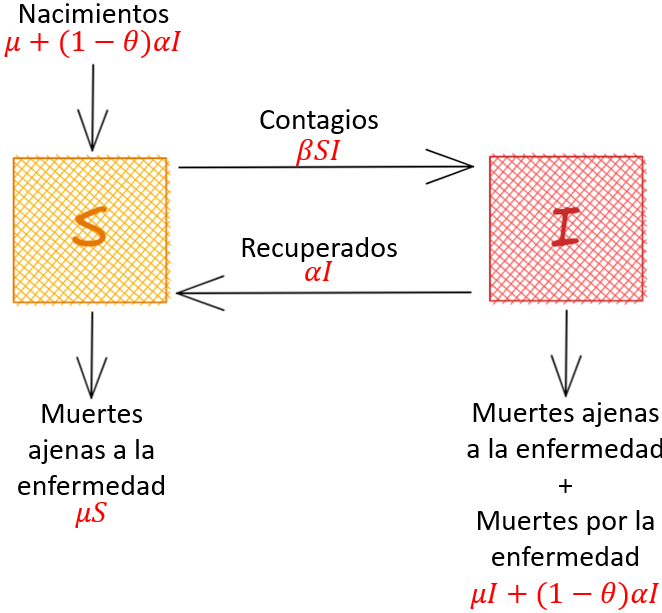
\includegraphics[width=0.7\textwidth]{Imagenes/SIS_compartimientos.PNG}
  \caption{El modelo SIS}
  \label{fig:SIS}
\end{figure}
\end{minipage}
\hfill
\begin{minipage}{0.5\textwidth}
\begin{figure}[h]
  \centering
    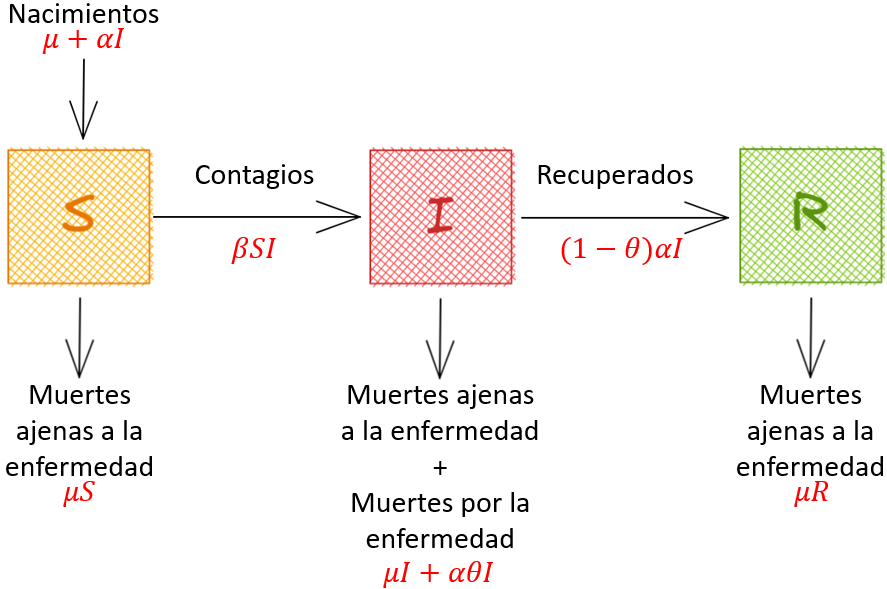
\includegraphics[width=1\textwidth]{Imagenes/SIR_compartimientos.PNG}
  \caption{El modelo SIR}
  \label{fig:SIR}
\end{figure}
\end{minipage}\\
Vistos como ecuaciones diferenciales:\\
\begin{minipage}{0.48\textwidth}
\begin{equation*}\label{eq:modeloSIS}
\left\{
\begin{array}{l}
S' = \mu(1 - S) + (1 - \theta)\alpha I - \beta S I, \\
I' = \beta S I - (1 - \theta)\alpha I - \mu I.
\end{array}
\right.
\end{equation*}

\end{minipage}
\hfill
\begin{minipage}{0.48\textwidth}
\begin{equation*}\label{eq:Modelo SIR}
\left\{
\begin{array}{l}
S' = \mu(1 - S) + \alpha\theta I - \beta S I, \\
I' = \beta S I - \alpha I - \mu I\text{, y } \\
R' = \alpha I - \alpha\theta I - \mu R.
\end{array}
\right.
\end{equation*}
\end{minipage}\\
Donde el indicador $\mathcal{R}_0$ para cada modelo es:\\
\begin{minipage}{0.48\textwidth}
$$\mathcal{R}_0 = \frac{\beta}{\alpha(1-\theta)+\mu}$$
\end{minipage}
\hfill
\begin{minipage}{0.48\textwidth}
$$\mathcal{R}_0 = \frac{\beta}{\alpha+\mu}.$$
\end{minipage}
\end{frame}

\subsection{Topología}
\begin{frame}{Topología}
\textbf{Definición:} Sean $X$ un espacio topológico y $x\in X$. Diremos que un subconjunto $V$ de $X$ es una \textit{vecindad} de $x$, si existe un abierto $A$ tal que $x\in A\subseteq V$. Denotaremos por $\mathcal{V}(x)$ a la familia de todas las vecindades de $x$.

\textbf{Definición:} Para un punto $x$ en un espacio topológico $X$, un subconjunto $\mathcal{B}(x)$ de $\mathcal{V}(x)$ es un \textit{sistema fundamental de vecindades de $x$} sí para cada $V\in\mathcal{V}(x)$, existe $B\in\mathcal{B}(x)$ tal que $B\subseteq V$. 

\textbf{Definición:} Una \textit{vecindad minimal de} $x$ es la intersección de todas las vecindades de $x$. Lo denotaremos como $U_x$.

\textbf{Definición:} Un espacio topológico $X$ que tiene un sistema fundamental de vecindades numerable en cada uno de sus puntos se dice que satisface el primer axioma de numerabilidad o simplemente que es uno-numerable.
\end{frame}

\subsection{Autómatas celulares}
\begin{frame}{Autómatas celulares}
Podemos pensar en un autómata celular como un conjunto de células que tienen diferentes comportamientos en el tiempo y que interactúan entre sí, de la misma manera que en sistema biológico de donde se obtiene su nombre.

Un \textbf{espacio de células} $\mathcal{L}$ es el conjunto donde viven e interactúan todas las células que se consideran para el modelo. En general este espacio es discreto, regular y finito.%, esto último debido a las limitaciones computacionales presentes en las herramientas con las que se construyen los modelos en autómatas celulares.

El \textbf{conjunto de estados} $\Sigma$ es el conjunto finito de todas las posibles categorías en las que pueden estar las células del espacio $\mathcal{L}$. %Cada elemento $\sigma$ de $\Sigma$ será conocido como un estado del modelo.

Las \textbf{reglas} que rigen el comportamiento de los estados de las células depende del estado de sus vecinos y su asignación puede ser de dos posibles tipos: determinística o totalística, y se deben aplicar en simultáneo sobre cada una de las células.
\end{frame}

\begin{frame}{Autómatas celulares: Reglas de evolución}
\textbf{Reglas determinísticas}\\
\begin{minipage}{0.65\textwidth}
\begin{figure}[h]
  \centering
    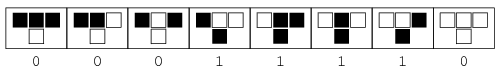
\includegraphics[width=1\textwidth]{Imagenes/regla30.PNG}
  \caption{Regla 30 de Wolfram. Captura tomada de \cite{rule30}}
  \label{fig:Regla30}
\end{figure}
\end{minipage}
\hfill
\begin{minipage}{0.3\textwidth}
\begin{figure}[h]
  \centering
    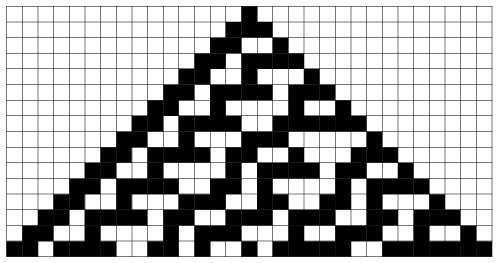
\includegraphics[width=0.8\textwidth]{Imagenes/regla30en15.PNG}
  \caption{Evolución del espacio en 15 iteraciones.}
  \label{fig:Regla30}
\end{figure}
\end{minipage}\\

\textbf{Reglas totalísticas}
    
%Las reglas totalísticas no establecen una correspondencia directa entre estados y combinaciones de vecindades, sino que en su lugar utilizan un componente probabilístico. %Esto significa que dependiendo de la combinación, la célula sobre la que se aplica la regla puede tomar un estado de un subconjunto del conjunto de estados $\Sigma$. 
    
%Existe un subtipo de este tipo de reglas conocido como las reglas semi-totalísticas, en las que el subconjunto que se considera para la evolución de la célula sobre la que se aplica la regla, depende del estado de la misma célula. De ese modo, definimos una regla semi-totalística como:
    
\begin{align*}
    \phi:\Sigma_x\times\overbrace{\Sigma\times\Sigma\times\cdots\times\Sigma}^{N}&\longrightarrow \left\{ \begin{array}{cc}
    \sigma_1 \subseteq \Sigma_x & \text{si el estado de }x\text{ es }s_1 \\
    \sigma_2 \subseteq \Sigma_x & \text{si el estado de }x\text{ es }s_2 \\
    \vdots & \vdots \\
    \sigma_k \subseteq \Sigma_x & \text{si el estado de }x\text{ es }s_k
    \end{array} \right. ,
\end{align*}
    
donde $k$ es la cantidad de posibles estados que puede tomar $x$.
\end{frame}

\begin{frame}{Autómatas celulares: Sistemas de vecindades}
En general no se trabaja con todo el conjunto $\mathcal{V}(x)$ sino que se consideran elementos de cada una de estas familias para conformar un conjunto de vecindades sobre el espacio $\mathcal{L}$. Este conjunto se conoce como un \textbf{sistema de vecindades} sobre $\mathcal{L}$.

\begin{figure}[h]
  \centering
    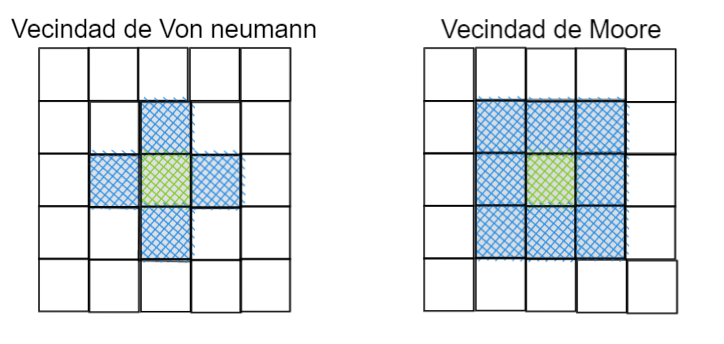
\includegraphics[width=0.48\textwidth]{Imagenes/vecindades.PNG}
  \caption{Vecindades usuales para autómatas celulares}
  \label{fig:Moore - Von neumann}
\end{figure}    

De ese modo, un \textbf{autómata celular} es una la tupla de la forma  $A=(\mathcal{L},\Sigma,\mathcal{N}(\mathcal{L}),\phi)$ con $\mathcal{N}(\mathcal{L})$ un sistema de vecindades sobre $\mathcal{L}$.
\end{frame}

\section{Modelos epidemiológicos en autómatas celulares}
\subsection{Relaciones entre células}
\begin{frame}{Relaciones entre células}
Pensemos por un momento en que si un individuo susceptible a una enfermedad tiene contacto con muchos infectados, puede enfermarse con mucha más facilidad que un individuo que tiene contacto con pocos infectados. Ahora bien \textbf{¿cuántas interacciones con infectados de todos las que puede llegar a tener una célula, son suficientes para generar una probabilidad de contagio considerable?}

A diferencia del trabajo realizado en "\textit{Epidemiological modeling with a population density map-based cellular automata simulation system}" \cite{populationDensity} en el que cada celda representaba una región, consideraremos a cada división como un único individuo que será dotado de un conjunto de cualidades como el estado de salud, la edad, los vecinos, etc.
\end{frame}

\begin{frame}{Relaciones entre células}
Denotaremos la relación entre células con el símbolo $\thicksim$ y una vez dicho esto tenemos que:

\begin{itemize}
    \item Todas las células están en contacto con ellas mismas, por lo que para cada célula $x$ se cumple $x \thicksim x$.
    \item Si una célula estuviera en contacto con alguna otra entonces esa célula estaría en contacto con la primera, es decir, $x\thicksim y$ implica $y\thicksim x$.
    \item Si una célula interactúa con otras dos no implica necesariamente que estas interactúen entre sí, por lo que $x\thicksim y$ y $x\thicksim z$ no implican que $y\thicksim z$.
\end{itemize}
\end{frame}

\begin{frame}{Relaciones entre células: Grados de impacto}
\textbf{Definición:} Denotaremos como $a\thicksim_n b$ con $n\in\mathbb{N}$, a la menor cantidad de interacciones entre $a$ y $b$. Conoceremos como \textbf{grado de impacto} a la relación $\thicksim_n$.

Consideremos el siguiente ejemplo en donde $\mathcal{A}=\{\emptyset,\{a\},\{b\}.\{a,b\},\{a,c\},\{a,b,c\}\}$:

$$\begin{array}{cccccccc}
    a\thicksim_0 a, & b\thicksim_0 b, & a\thicksim_1 c, & a\thicksim_1 b, &
    b\thicksim_1 a, & b\thicksim_2 c, & c\thicksim_0 a, & c\thicksim_0 c
\end{array}$$
\begin{figure}[h]
  \centering
    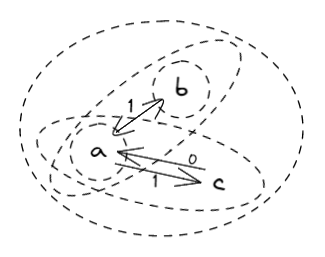
\includegraphics[width=0.3\textwidth]{Imagenes/grados_de_impacto.PNG}
  \caption{Grados de impacto para el espacio $X$ con la topología $\mathcal{A}$.}
  \label{fig:gradoImpacto}
\end{figure}
\end{frame}

\begin{frame}{Relaciones entre células: Grados de impacto}
%De la definición de grado de impacto podemos deducir el siguiente resultado:

\textbf{Teorema:} Los grados de impacto de una célula $x$ definen un sistema fundamental de vecindades.

\underline{\textit{Demostración:}}
\begin{enumerate}
    \item Para $x\in\mathcal{L}$ defina recursivamente a los conjuntos $\mathcal{A}_k$ formados por los elementos son los puntos con grado de impacto $k$ con $x$.
    \item Se observa que $A_i\subseteq A_j$ para $0\leq i\leq j$ y de ese modo $A_i\in\mathcal{V}(x)$ para $i=0,1,\cdots,n$
    \item Se comprueba que $A_0$ es la vecindad mínimal de $x$. (se contradice la definición de $\thicksim_n$)
    \item Para $y\in A_0$ se afirma que $x$ e $y$ no son separables por lo que $y\in\mathcal{V}(x)$ y con esto existe un abierto que está en todos los $V\in\mathcal{V}(x)$.
\end{enumerate}

\textbf{Proposición:} Sea $x\in\mathcal{L}$ una célula y sea $\mathcal{A}$ la familia de conjuntos encajados definidos por el grado de impacto con $x$. Entonces:
\begin{enumerate}
    \item El conjunto $\mathcal{A}$ posee elemento mínimal igual a $A_0$,
    \item $\mathcal{A}$ es un conjunto ordenado finito con el orden de la contenencia, y
    \item $\mathcal{L}$ es un espacio uno-numerable.
\end{enumerate}

%Algo que debemos tener en cuenta es que el grado de impacto por si solo no nos proporciona una medida del impacto que tienen los cambios de estado de células "lejanas" (o de grado de impacto mayor a cero). Estas medidas de impacto se entenderán como la probabilidad de que un cambio de estado afecte a la célula con la que estamos realizando la comparación. De ese modo, las tasas de impacto serán valores entre 0 y 1 que pueden venir dados por cualquier tipo de función que tenga como dominio al conjunto de grados de impacto.
\end{frame}

\begin{frame}{Reglas de evolución: Tasas de impacto}
El grado de impacto por si solo no nos proporciona una medida del impacto que tienen los cambios de estado de células "lejanas" (o de grado de impacto mayor a cero). 

Estas medidas de impacto se entenderán como la probabilidad de que un cambio de estado afecte a la célula con la que estamos realizando la comparación. De ese modo, las tasas de impacto serán valores entre 0 y 1 que pueden venir dados por cualquier tipo de función que tenga como dominio al conjunto de grados de impacto.
\end{frame}

\subsection{Reglas de evolución}

\begin{frame}{Reglas de evolución: Notación}
Dado que estamos trabajando sobre poblaciones de tamaño constante la manera en la que interpretaremos el nacimiento de una célula será con la ocupación del espacio que deja una que muere. 

Identificaremos a los espacios que dejan las células que mueren con el estado $D$, esto nos permitirá separar a los espacios que pueden ocuparse y los que no de células que interactúen con sus vecinos. 

Al igual que en los modelos clásicos, asumiremos que los individuos que "nacen" son susceptibles a la enfermedad.
\end{frame}

\begin{frame}{Reglas de evolución: Notación}
Antes de comenzar a definir nuestras reglas de evolución definiremos las siguientes notaciones:
\begin{itemize}
    \item El estado de la célula $x$ en un momento $t$ se denotará como $\pi^t(x)$.
    \item La cantidad de individuos con grado de impacto $g$ y estado $K$ de una célula $x$ en un momento $t$, será representado como $\sigma_{g,K}^t(x)$.
    \item Para representar a la cantidad de individuos con un grado de impacto $g$ usaremos el símbolo $\Delta_g$. 
    \item Usaremos los símbolos $\mathcal{S}^t,\mathcal{I}^t,\mathcal{R}^t$ y $\mathcal{D}^t$ para denotar a los conjuntos de células susceptibles, infectadas, recuperadas y muertas respectivamente en el espacio $\mathcal{L}$ en el tiempo $t$. Con lo cual
    $$\mathcal{S}^t=\{x\in\mathcal{L}:\pi^t(x)=S\},$$
    y de manera análoga se definen los conjuntos $\mathcal{I}^t,\mathcal{R}^t$ y $\mathcal{D}^t$. Note que $$\mathcal{S}^t\cup\mathcal{I}^t\cup\mathcal{R}^t\cup\mathcal{D}^t=\mathcal{L}\text{ para todo tiempo }t.$$
\end{itemize}
\end{frame}

\begin{frame}{Reglas de evolución: Modelo SI}
\textbf{Ejemplo:}

\begin{minipage}{0.55\textwidth}
\begin{figure}[h]
  \centering
    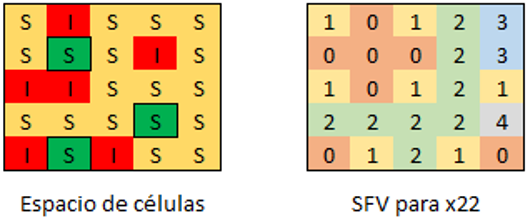
\includegraphics[width=0.8\textwidth]{Imagenes/cellSpacePresentation.png}
    \caption{Configuración inicial de estados y sistemas fundamentales de vecindades}
    \label{fig:configuraciónInicialEspacio25Celulas}
\end{figure}
\end{minipage}
\hfill
\begin{minipage}{0.4\textwidth}
\begin{figure}[h]
  \centering
    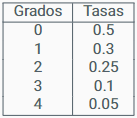
\includegraphics[width=0.5\textwidth]{Imagenes/RelacionTasasYGrados_Ex_SI.png}
    \caption{Relación entre tasas y grados de impacto.}
\end{figure}
\end{minipage}

\begin{align*}
    \begin{array}{l}
        \sum_g\sigma_{g,S}^0(x_{2,2})\cdot P(g) = 4\cdot0.5+6\cdot0.3+6\cdot0.25+2\cdot0.1+1\cdot0.05 = 5.55 \\
        \sum_g\sigma_{g,I}^0(x_{2,2})\cdot P(g) = 3\cdot0.5+1\cdot0.3+2\cdot0.25+0\cdot0.1+0\cdot0.05 = 2.3\\
        i_{2,2}(0) = \frac{\beta}{\alpha}\cdot\left(\frac{3\cdot0.5}{7}+\frac{1\cdot0.3}{7}+\frac{2\cdot0.25}{8}+\frac{0\cdot0.1}{2}+\frac{0\cdot0.05}{1}\right)=\frac{179}{560}\cdot\frac{\beta}{\alpha}
    \end{array}
\end{align*}
Para una tasa $\beta=0.5$ y una tasa $\alpha=0.2$ se tiene que $i_{2,2}(0)=0.8$.
\end{frame}

\begin{frame}{Reglas de evolución: Modelo SI}
\textbf{Definición:} Para una célula $x$ en un espacio $\mathcal{L}$ definimos la regla SI como:
\begin{equation}
    \phi_{SI}^t(x)=\left\{\begin{array}{ll}
        S & \text{si }\pi^t(x)=S\text{, }\sum_g{\sigma_{g,I}^t(x)\cdot P(g)}\leq \sum_g{\sigma_{g,S}^t(x)\cdot P(g)}\text{ y }\rho\geq i(t),\\
        \pi^t(x) & \text{si }\pi^t(x)\notin\{S,I\}\text{,} \\
        I & \text{en otro caso,}
    \end{array}\right.
\end{equation}
con $\rho\in\mathcal{U}_{[0,1]}$, $P(g)$ la tasa de impacto del grado $g$ e
\begin{equation}
    i(t) = \frac{\beta}{\alpha}\sum_g{\frac{\sigma_{g,I}^t(x)}{\Delta_g}}\cdot P(g),
\end{equation}
donde el factor $\frac{\beta}{\alpha}$ indica la afectación ocasionada por la enfermedad y el factor restante corresponde al comportamiento de las células y su impacto en la célula $x$.

\textbf{Nota:} Se espera que en futuras investigaciones se profundice en cambios sobre la distribución usada, esto vendrá dado por el contexto del problema planteado.
\end{frame}

\begin{frame}{Reglas de evolución: Modelos SIS y SIR}
\textbf{Definición:} Dada una célula $x$ en un conjunto $\mathcal{L}$ definimos respectivamente las reglas de evolución para los modelos SIS y SIR respectivamente como:
\begin{equation}
    \phi_{SIS}^t(x)=\left\{\begin{array}{ll}
        \phi_{SI}^t(x) & \text{si }\pi^t(x) = S,\\
        I & \text{si }\pi^t(x)=I\text{ y }\rho>\alpha,\\
        S & \text{si }\pi^t(x)=I\text{ y }\rho\leq\alpha.
    \end{array}\right.
\end{equation}

\begin{equation}
    \phi_{SIR}^t(x)=\left\{\begin{array}{ll}
        \phi_{SI}^t(x) & \text{si }\pi^t(x) = S,\\
        I & \text{si }\pi^t(x)=I\text{ y }\rho>\alpha,\\
        R & \text{si }\pi^t(x)=I\text{ y }\rho\leq\alpha, y \\
        R & \text{si }\pi^t(x)=R,
    \end{array}\right.
\end{equation}
donde $\rho\in\mathcal{U}_{[0,1]}$.
\end{frame}

\begin{frame}{Reglas de evolución: Modelos SIS y SIR}
\begin{minipage}{0.5\textwidth}
\begin{figure}[h]
  \centering
 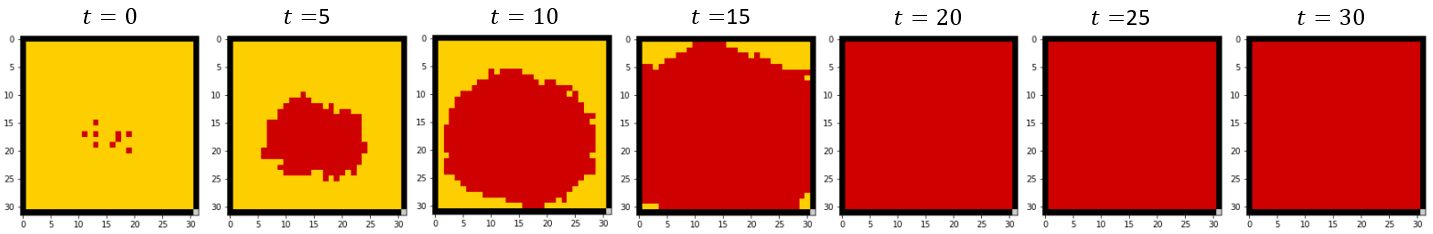
\includegraphics[width=1\textwidth]{Imagenes/sisEn30.PNG}
 \caption{Evolución de la enfermedad en 30 días (modelo SIS).}
 \label{fig:sisEn30}
\end{figure}
\begin{figure}[h]
  \centering
 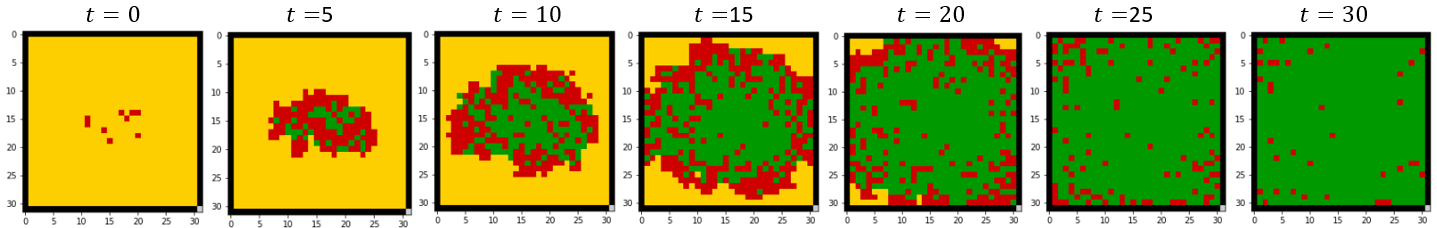
\includegraphics[width=1\textwidth]{Imagenes/sirEn30.PNG}
 \caption{Evolución de la enfermedad en 30 días (modelo SIR).}
 \label{fig:sirEn30}
\end{figure}
\end{minipage}
\hfill
\begin{minipage}{0.45\textwidth}
\begin{figure}[h]
  \centering
    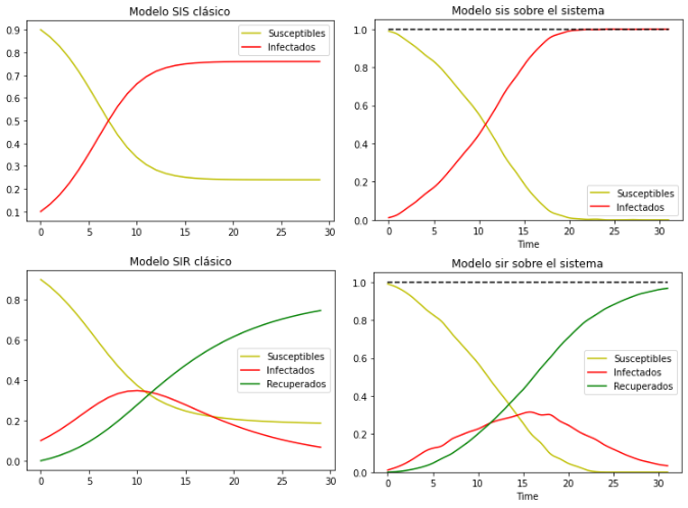
\includegraphics[width=1\textwidth]{Imagenes/solucionesSISySIR1.PNG}
    \caption{Evolución de la enfermedad en 30 días (modelos clásicos vs reglas de evolución).}
    \label{fig:sirEn30}
\end{figure}
\end{minipage}
\end{frame}

\begin{frame}{Reglas de evolución: Modelos con natalidad y mortalidad}
Para estos modelos se considerarán las "edades" de las células, por lo que
$$Dom(\phi_\mu)=\Sigma_x\times K\times\overbrace{\Sigma\times\cdots\times\Sigma}^N\text{, con }K=\{1,2,\cdots,100\},$$
$$Ran(\phi_\mu)=\Sigma_x\times K.$$

\textbf{Definición:} Definimos la regla de evolución con nacimientos y muertes para $M$ como:
\begin{equation*}
    \mu_{M,T}^t(x)=\left\{\begin{array}{ll}
        D,0 & \text{si }t\not\equiv 0 \text{ (modulo }T\text{), }\pi^t(x)\in\{S,I,R\}\text{ y }\rho\leq\omega_k, \\
        D,0 & \text{si }\pi^t(x)=D\text{ y }\rho>b,\\
        S,1 & \text{si }\pi^t(x)=D\text{ y }\rho\leq b,\\
        \phi_M^t(x),E^t(x) & \text{si }t\not\equiv 0 \text{ (modulo }T),\\
        \phi_M^t(x),E^t(x)+1 & \text{si }t\equiv 0 \text{ (modulo }T),
    \end{array}\right.
\end{equation*}
donde $\omega_k$ es la probabilidad de morir por causas ajenas a la enfermedad para las edades en la k-ésima partición del intervalo $[0,100]$, $b$ es la tasa de natalidad, $\phi_M^t$ es la regla de evolución del modelo epidemiológico, $E^t(x)$ denota la edad de la célula $x$ en el momento $t$ y $\rho\in\mathcal{U}_{[0,1]}$.
\end{frame}

% \begin{frame}{Reglas de evolución: Modelos con natalidad y mortalidad}
% Consideremos una probabilidad de nacimiento (u ocupación de espacios disponibles) $b=0.02$ y una unidad temporal $T=2$ sobre la siguiente configuración de estados en un espacio de células junto con las probabilidades de muerte por grupo de edad: 

% \begin{figure}[h]
%   \centering
%     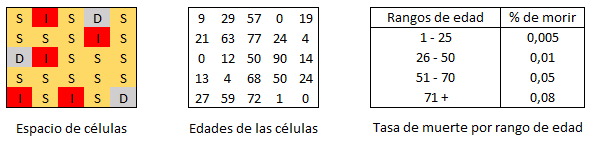
\includegraphics[width=0.8\textwidth]{Imagenes/conInicialMNM.PNG}
%     \caption{Configuración inicial para el espacio de células y tasas de muerte por edad.}
%     \label{ex:configuraciónInicialNatalidadyMortalidad}
% \end{figure}
% \begin{figure}[h]
%   \centering
%     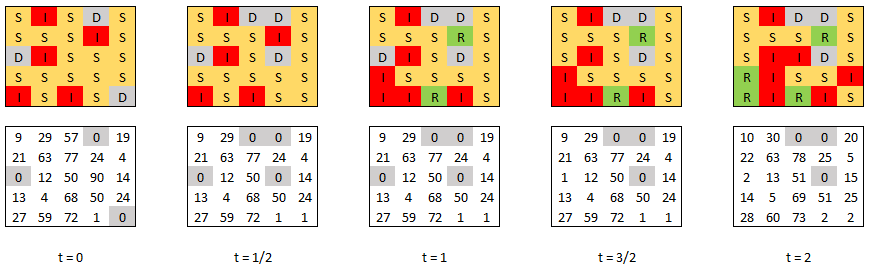
\includegraphics[width=1\textwidth]{Imagenes/natalidadMortalidad.PNG}
%     \caption{Aplicación de la regla $\mu_{SIR,2}^t(x)$}
%     \label{ex:aplicaciónReglaNatalidadyMortalidad}
% \end{figure}
% $\beta=0.05$ y $\alpha=0.2$, $\mu=\frac{1}{75\cdot6}$
% \begin{figure}[h]
%   \centering
%     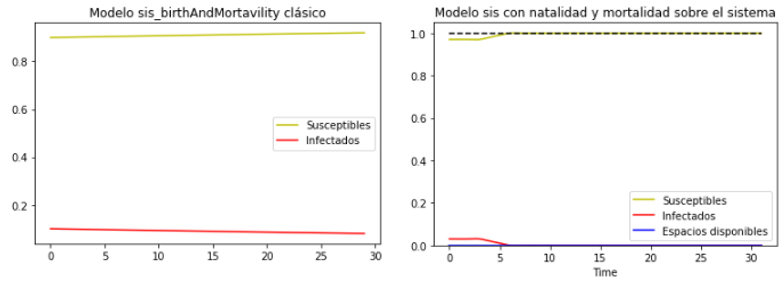
\includegraphics[width=0.75\textwidth]{Imagenes/solucionesNatalidadYMortalidad.PNG}
%     \caption{Evolución de la enfermedad en 30 bimestres (modelo clásico y regla $\mu_{SIS,6}^t(x)$)}
%     \label{ex:aplicaciónReglaNatalidadyMortalidad}
% \end{figure}
% \end{frame}

\begin{frame}{Reglas de evolución: Modelos con muerte por enfermedad}
\textbf{Definición:} Sea $x$ una célula en un conjunto $\mathcal{L}$, $M$ un modelo epidemiológico ($SIS$, $SIR$, etc.) y $T$ una unidad temporal (días, meses, años, etc.). Definimos la regla de evolución con muerte por enfermedad para $M$ como:
\begin{equation}
    \theta_{M,T}^t(x)=\left\{\begin{array}{ll}
        D,0 & \text{si }\pi^t(x)=I\text{ y }\rho\leq\theta_k, \\
        \mu_{M,T}^t(x) & \text{en otro caso.}
    \end{array}\right.
\end{equation}
Donde $\theta_k$ es la probabilidad de morir por la enfermedad para los individuos con una edad en el intervalo k-ésimo de la partición del intervalo $[0,100]$, $\mu_{M,T}^t$ es la regla de evolución para modelos con nacimientos y muertes y $\rho\in\mathcal{U}_{[0,1]}$.
% Partiremos de la misma configuración de edades sobre un sistema de 100 células y las mismas tasas de natalidad y mortalidad consideradas en el ejemplo \ref{ex:aplicaciónReglaNatalidadyMortalidad}. Tomaremos las vecindades de Von Neumann para describir sus interacciones. En cuanto a la enfermedad, supondremos una tasa de infección $\beta=0.5$, una de recuperación $\alpha=0.2$ y una probabilidad de muerte causada por la misma enfermedad de $\theta=0.4$ (tomamos este valor con el objetivo de comparar los resultados con el modelo clásico).

% \begin{figure}[h]
%   \centering
%     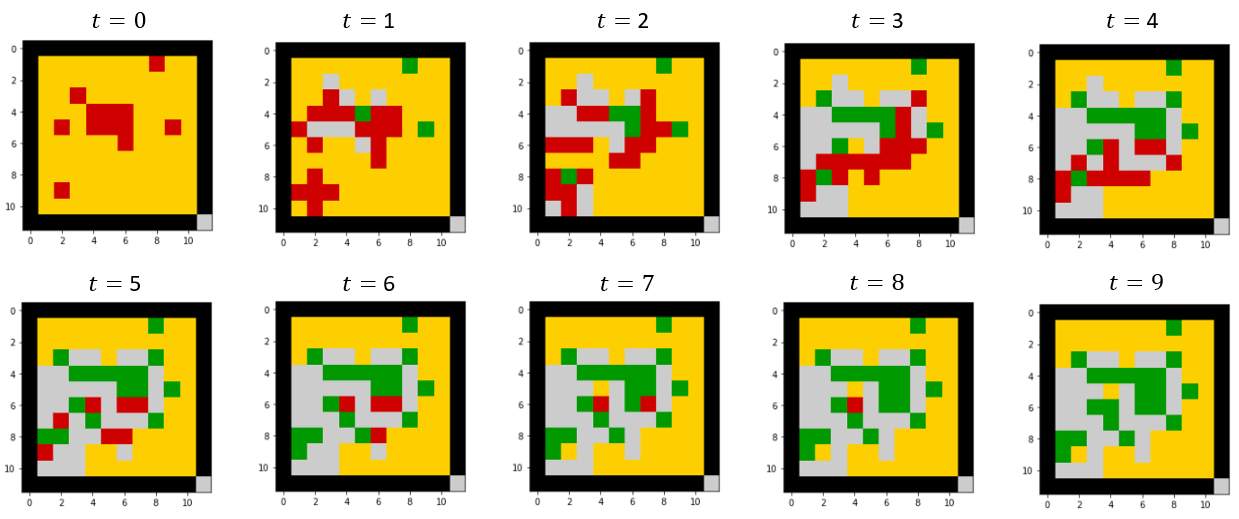
\includegraphics[width=1\textwidth]{Imagenes/evolucionesMuertePorEnfermedad.PNG}
%     \caption{Aplicación de la regla $\theta_{SIR,6}^t(x)$ en 10 iteraciones}
%     \label{fig:muertePorEnfermedad10Veces}
% \end{figure}
\end{frame}

\section{Ejemplo particular}
\begin{frame}{Ejemplo particular}
\begin{itemize}
    \item \textbf{Escuela (E):} Se sabe que en el pueblo hay 9 niños y 2 profesores.
    \item \textbf{Oficinas (O):} Cuenta con un personal de 16 individuos.
    \item \textbf{Mercado (M):} Se identificaron 8 trabajadores.
    \item \textbf{Hospital (H):} Entre doctores, enfermeros y pacientes se identifica una cantidad de 14 individuos. Para un total de 49 personas en el pueblo.
\end{itemize}
\begin{minipage}{0.48\textwidth}
\begin{figure}[h]
  \centering
    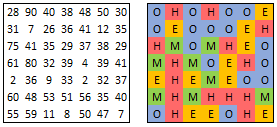
\includegraphics[width=0.7\textwidth]{Imagenes/edadesYOcupaciones.PNG}
    \caption{Edades y ocupaciones en el pueblo.}
    \label{fig:edadesYOcupaciones}
\end{figure}
\end{minipage}
\hfill
\begin{minipage}{0.48\textwidth}
\begin{figure}[h]
  \centering
    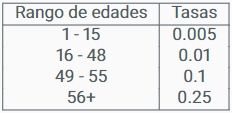
\includegraphics[width=0.65\textwidth]{Imagenes/tasasDeLetalidad_ex_Pueblo.png}
    \caption{Tasas de letalidad de la gripa.}
\end{figure}
\end{minipage}

En el caso de la enfermedad, tomaremos $\alpha=\frac{1}{5}=0.2$ (la gripa dura en promedio 5 días), $\beta=0.3$, tasas de natalidad del $2\%$ y de mortalidad del $0.5\%$. Supondremos inicialmente que la enfermedad inicia en el hospital.
\end{frame}

\begin{frame}{Ejemplo particular}
\begin{figure}[h]
  \centering
    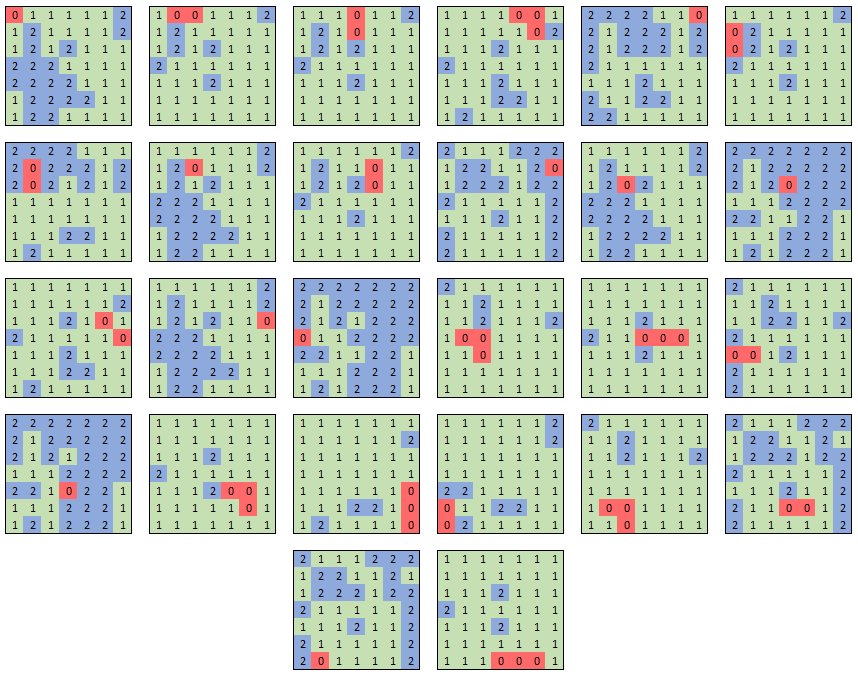
\includegraphics[width=0.8\textwidth]{Imagenes/vecindadesCap4.PNG}
    \caption{Grados de impacto.}
    \label{fig:GradosdeImpactoEX4}
\end{figure}
\end{frame}

\begin{frame}{Ejemplo particular}
Para un periodo de 30 días y las tasas de impacto $P(0)=1,P(1)=0.5$ y $P(2)=0.25$ se tiene el comportamiento descrito en la segunda figura:
\begin{figure}[h]
  \centering
    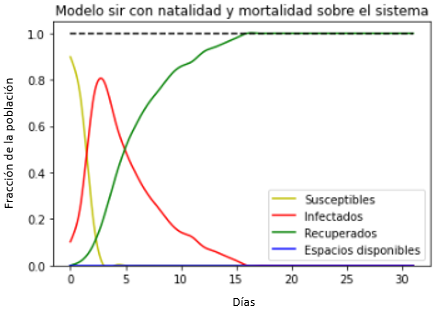
\includegraphics[width=0.5\textwidth]{Imagenes/metricas1.PNG}
    \caption{Cambios de estado con punto de inicio en el hospital.}
    \label{fig:metricas1}
\end{figure}
\end{frame}

\begin{frame}{Ejemplo particular}
En la siguiente figura podremos observar la evolución promedio sobre 100 simulaciones de la enfermedad teniendo en cuenta diferentes tasas de impacto:

\begin{figure}[h]
  \centering
    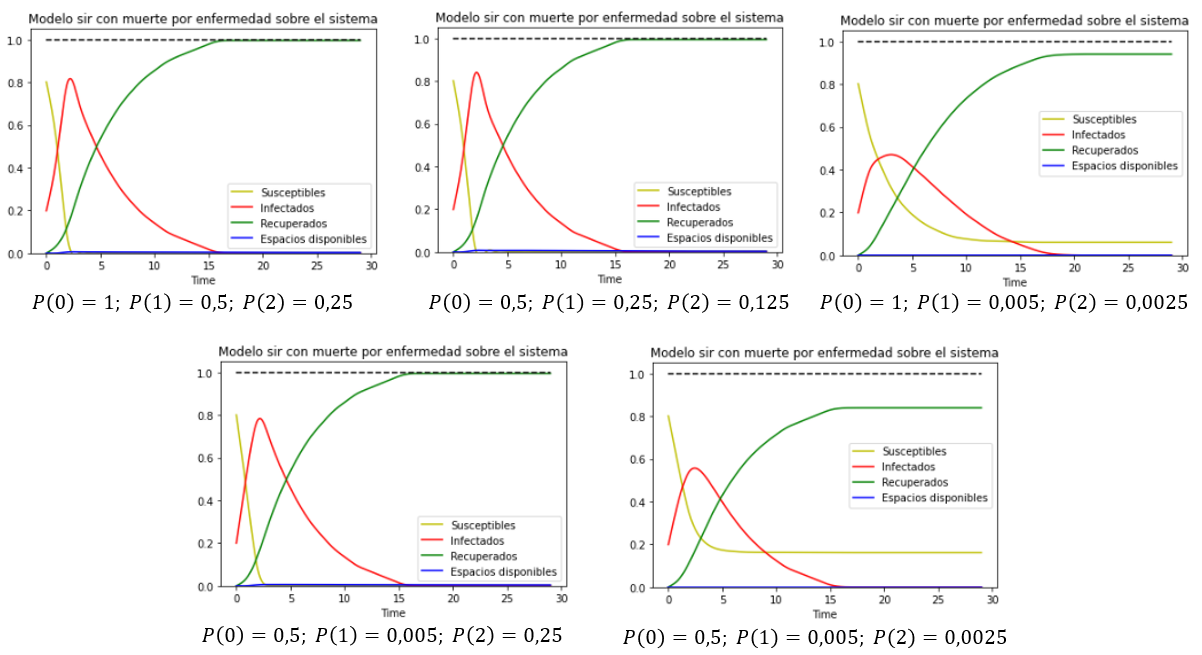
\includegraphics[width=1\textwidth]{Imagenes/comparacionTasasImpacto.PNG}
    \caption{Evolución promedio de la enfermedad tomando distintas tasas de impacto.}
    \label{fig:comparacionTasasdeImpacto}
\end{figure}
\end{frame}

\begin{frame}{Ejemplo particular}
Teniendo en cuenta que el ejemplo anterior muestra que diferentes tasas de impacto afectan a las curvas de evolución del modelo, podemos preguntarnos si ocurre algo similar con diferentes condiciones iniciales. 

\begin{figure}[h]
  \centering
    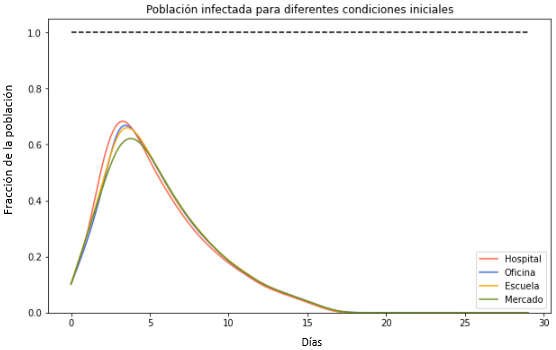
\includegraphics[width=0.5\textwidth]{Imagenes/condicionesIniciales.png}
    \caption{Población infectada por condición inicial.}
    \label{fig:condicionesIniciales}
\end{figure}
\end{frame}

\begin{frame}{Ejemplo particular}
Por otro lado, podemos también preguntarnos si el sistema de vecindades con el que se describen las interacciones, tiene algún tipo de incidencia en el comportamiento de la enfermedad. %Para responder a esta inquietud nos planteamos el escenario que se puede observar en la figura (\ref{fig:comparacionTasasdeImpacto}) en donde se muestra la evolución de la misma enfermedad, sobre un espacio en el que las relaciones entre células se pueden describir a partir de los sistemas de vecindades de Moore y de Von Neumann junto con el escenario planteado durante el presente capítulo. Para los tres escenarios se tomaron las curvas promedio sobre un total de 100 simulaciones.
\begin{figure}[h]
  \centering
    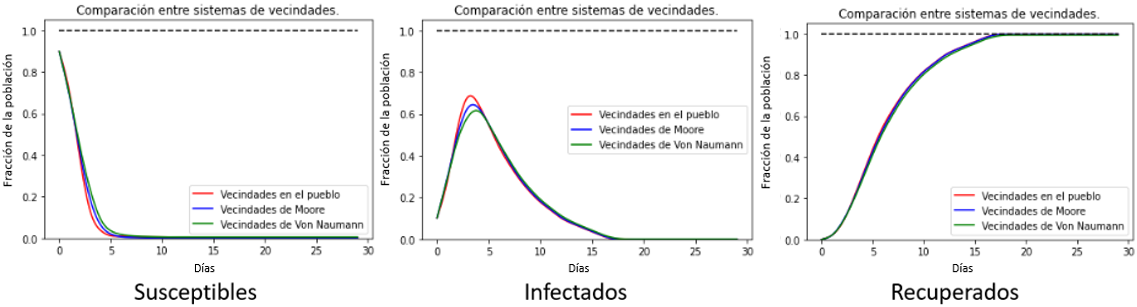
\includegraphics[width=1\textwidth]{Imagenes/comparacionSistemasVecindades.PNG}
    \caption{Evolución promedio de la enfermedad tomando tres sistemas de vecindades.}
    \label{fig:comparacionSistemasDeVecindades}
\end{figure}
\end{frame}

\section{Conclusiones}
\begin{frame}{Conclusiones}
\begin{itemize}
    \item Haciendo uso de las \textbf{propiedades de los autómatas celulares} para describir comportamientos espaciales y de los sistemas fundamentales de vecindades \textbf{es posible modelar las relaciones sociales} de un conjunto de individuos determinado.
    \item Las \textbf{condiciones iniciales} sobre cómo interactúan las células \textbf{no afectan a los puntos de equilibrio} de las curvas que describen el comportamiento de la enfermedad. Sin embargo, como se observa en los ejemplos realizados, los \textbf{cambios en la condición inicial} pueden afectar a la \textbf{velocidad de propagación} de la misma enfermedad.
    \item Se evidencia que limitar y/o reducir la intensidad de las interacciones sociales es una medida efectiva para disminuir los casos de individuos infectados.
\end{itemize}
\end{frame}

\begin{frame}{Conclusiones}
\begin{itemize}
    \item Las reglas y algoritmos propuestos \textbf{permiten visualizar de manera clara e intuitiva a la manera en la que una enfermedad evoluciona dentro de una población}, manteniendo un comportamiento que puede ser descrito en cierta medida por los modelos compartimentales clásicos.
    \item Si bien las reglas planteadas permiten analizar características que no eran posibles con los modelos clásicos, se evidencia una \textbf{limitación} en cuanto a que se asume una \textbf{capacidad máxima de individuos en el sistema.}
    \item La \textbf{metodología} empleada para el diseño e implementación de las reglas de evolución descritas en este trabajo, brindan un camino claro para la definición de reglas que modelen el comportamiento de modelos epidemiológicos más generales.
\end{itemize}
\end{frame}

\section{Referencias}
\begin{frame}[allowframebreaks]{Referencias}
\bibliographystyle{plain} % apalike
\bibliography{BibliMSc}
\end{frame}

\end{document}